% !TEX TS-program = XeLaTeX
%!TEX encoding = UTF-8 Unicode
%==================================================
%      PREAMBOLO e DICHIARAZIONI INIZIALI
%==================================================
\documentclass[10pt,oneside,a4paper]{article}

\usepackage[utf8]{inputenc} 
\usepackage[italian]{babel}
\usepackage[T1]{fontenc}
\usepackage{siunitx} %Inserisce automaticamente i dati con le unità  di misura correttamente formattate del SI (utilizzo: \SI{0.82}{m^2}, in generale \SI{misura con il punto decimale}{unità  di misura})
\sisetup{output-decimal-marker = {.}, separate-uncertainty = true, input-uncertainty-signs = \pm, detect-weight=true, detect-family=true} %per usare SI con il punto decimale
\usepackage{listings} %Per citare codice informatico formattandolo correttamente
\usepackage{amsmath,amsthm,verbatim,amssymb,amsfonts,amscd,graphicx,mathtools}
\usepackage[makeroom]{cancel}
\newcommand{\abs}[1]{\left\lvert\,#1\,\right\rvert}
\usepackage{geometry}
\usepackage{epigraph}
\usepackage{booktabs}	%tabelle migliorate
\usepackage{tablefootnote}	%note a piè di pagina in tabella
\usepackage{threeparttable} %tabella con note a piè di tabella
\usepackage{caption}	%descrizione per figure
\usepackage{dblfnote}
\usepackage{supertabular}
\usepackage{longtable}
\captionsetup{tableposition=top,figureposition=bottom,font=small} %setup descrizione
\usepackage{float}
\usepackage{esvect} %vettori
\usepackage{longtable} %tabelle lunghe
\usepackage[dvipsnames]{xcolor}
\definecolor{sepia}{HTML}{80002A}
\usepackage[colorlinks=true, citecolor=black, linkcolor=sepia, urlcolor=black]{hyperref}
\usepackage{mathrsfs}
\usepackage{circuitikz}
\tikzset{
  font={\fontsize{7pt}{12}\selectfont}}
\ctikzset{bipoles/resistor/height=0.2}
\ctikzset{bipoles/resistor/width=0.4}
\ctikzset{bipoles/diode/height=0.3}
\ctikzset{bipoles/diode/width=0.3}
\ctikzset{tripoles/american nand port/height=0.7}
\ctikzset{tripoles/american nand port/width=0.8}
\usepackage{enumitem} %Liste senza spazi verticali
\setlist{noitemsep}
\usepackage{amsmath}
\usepackage{hyperref}
%\usepackage{pst-optexp} %Diagrammi ottici
\usepackage{physics} %Ambienti utili
\usepackage{upgreek} %Per avere lettere greche non corsive, ex. \upbeta


\interfootnotelinepenalty=10000


\usepackage{multicol}
\newenvironment{Figure}
  {\par\medskip\noindent\minipage{\linewidth}}
  {\endminipage\par\medskip}

%\newcommand{\var}{\operatorname{var}}
%\newcommand{\cov}{\operatorname{cov}}


\usepackage{listings} %Per inserire codice
\lstdefinestyle{CStyle}{
    backgroundcolor=\color{backgroundColour},   
    commentstyle=\color{mGreen},
    keywordstyle=\color{magenta},
    numberstyle=\tiny\color{mGray},
    stringstyle=\color{mPurple},
    basicstyle=\footnotesize\ttfamily,
    breakatwhitespace=false,         
    breaklines=true,                 
    captionpos=b,                    
    keepspaces=true,                 
    numbers=left,                    
    numbersep=5pt,                  
    showspaces=false,                
    showstringspaces=false,
    showtabs=false,                  
    tabsize=2,
    language=C
}

\definecolor{color1}{RGB}{90,0,0} % Color of the article title and sections
\definecolor{color2}{RGB}{0,20,50} % Color of the boxes behind the abstract and headings
\definecolor{mGreen}{rgb}{0,0.6,0}
\definecolor{mGray}{rgb}{0.5,0.5,0.5}
\definecolor{mPurple}{rgb}{0.58,0,0.82}
\definecolor{backgroundColour}{rgb}{0.95,0.95,0.92}


%==================================================
%                  PRIMA PAGINA
%==================================================

\title{\textsc{\textbf{Esperienza 3}: Diffrazione di un fascio laser}}
\author{\small{G. Galbato Muscio} \and \small{F. Ghimenti} \and \small{L. Gravina} \and \small{L. Graziotto}}
\date{7 Maggio 2019}

\begin{document}
	\begin{figure}
		\centering
		
\includegraphics[scale=0.5, trim={2.8cm 8.9cm 0 9cm}, clip]{logo.png}
	\end{figure}
	\maketitle
	\begin{center} 
		\fbox{{\fontsize{12pt}{8mm}\textsc{Gruppo D1-1}}} \\
	\end{center}
\hrule
\vfill
\renewcommand{\abstractname}{Abstract}
\begin{abstract}
Si misura la lunghezza d'onda della luce emessa da un laser He-Ne mediante lo studio della figura di diffrazione da una fenditura lineare e da un'apertura circolare in regime di Fraunhofer. Si verifica poi la validità del principio di Babinet studiando la figura di diffrazione in regime di Fraunhofer da un capello, e si stima il diametro dello stesso.
\end{abstract}
\vfill
\tableofcontents %Indice
\newpage


\pagebreak


\begin{multicols}{2}
%==================================================
%             APPARATO STRUMENTALE
%==================================================
\section{Apparato strumentale}

Si utilizza un laser He-Ne di lunghezza d'onda, dichiarata dal costruttore, $\lambda = \SI{632.8}{nm}$, montato su tavolo ottico\footnote{Si confronterà dunque il risultato sperimentale ottenuto in seguito con questo valore.}. 

In serie al laser è posta un'iride, allo scopo di evitare l'ingresso nel laser dei fasci di ritorno, che ne perturberebbero il comportamento. Due specchi orientati a \SI{45}{\degree} portano il fascio ad incidere sulla fenditura o sull'apertura circolare o sul capello; quindi, a distanza\footnote{L'incertezza associata è pari al doppio della risoluzione del metro a nastro, in quanto si ha un errore dovuto sia al posizionamento di un capo dello strumento, sia al posizionamento dell'altro.} $L = \SI{90.0 \pm 0.2}{cm}$, è posto il fotodiodo, montato su una slitta micrometrica di portata \SI{15}{mm} e risoluzione \SI{0.010}{mm}, che può essere traslato per misurare l'intensità luminosa delle frange di diffrazione.

La configurazione utilizzata è illustrata in Figura~\ref{fig:diagram}.

\begin{Figure}
	\begin{center}
	\hbox{\hspace{-0.8cm}
	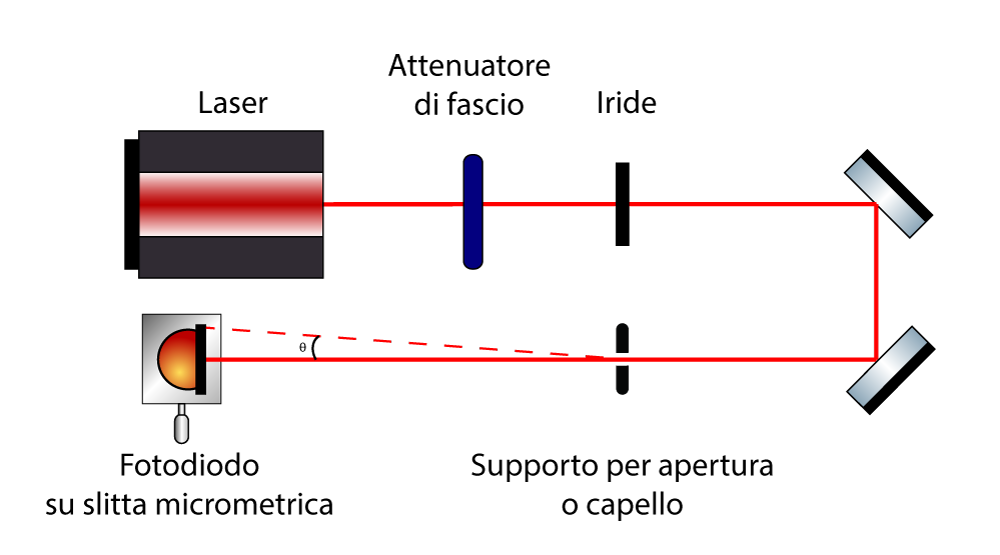
\includegraphics[width=1.1\linewidth]{diagram.png}}
	\captionof{figure}{Configurazione utilizzata.}
	\label{fig:diagram}
	\end{center}
\end{Figure}

Il segnale in uscita dal fotodiodo è misurato con il multimetro \texttt{METEX M-4650}. Le misure di intensità luminosa vengono riportate come differenza di potenziale misurata ai capi del fotodiodo, pertanto è da intendere la presenza di un fattore di proporzionalità non noto. Inoltre, si regola con un filtro attenuatore l'intensità della luce emessa dal laser in modo da restare all'interno della regione di linearità del fotodiodo, ossia al di sotto di \SI{10}{V}. L'incertezza associata alla misura dipende dall'oscillazione delle cifre riportate sul multimetro: l'errore sarà attribuito in modo da comprendere l'intervallo di variabilità di tali cifre. 

Poiché il fotodiodo permette l'ingresso della luce attraverso un foro di diametro circa \SI{200}{\micro m}, si compiranno spostamenti della slitta micrometrica di almeno \SI{100}{\micro m}, e pertanto l'incertezza associata alla posizione del fotodiodo sarà di \SI{100}{\micro m}.


\section{Misura della lunghezza d'onda}
Si utilizzano nel seguito fenditure di larghezza, assunta priva di incertezza, $b = (\SI{150}{\micro m}, \SI{200}{\micro m}, \SI{300}{\micro m}, \SI{400}{\micro m})$ e aperture circolari di diametro, assunto privo di incertezza, $d = (\SI{100}{\micro m}, \SI{200}{\micro m}, \SI{300}{\micro m})$; si allinea l'apparato sperimentale in modo da mantenere il fascio laser ad una altezza di circa \SI{14}{cm} dal banco ottico. Servendosi della vite micrometrica della slitta su cui è posto il fotodiodo, si misura il punto $x_0$ corrispondente al massimo della figura di diffrazione, e quindi si misura la distanza dello stesso dai punti corrispondenti ai minimi di ordine $m$.

Sono note le relazioni che legano ordine del minimo, angolo di osservazione e dimensione caratteristica dell'apertura
\[
\begin{aligned}
\sin\theta &= m\frac{\lambda}{b} \\
\sin\theta &= c(m)\frac{\lambda}{d}
\end{aligned}
\]
dove la prima è riferita alla fenditura e la seconda all'apertura circolare; $c(m)$ è un opportuno coefficiente legato alla funzione di Bessel. Per piccoli angoli $\theta$, si può approssimare $\sin\theta \simeq \tan\theta = (x-x_0) / L$, pertanto
\[
\begin{aligned}
\frac{x-x_0}{L} &= m\frac{\lambda}{b} \\
\frac{x-x_0}{L} &= c(m)\frac{\lambda}{d}.
\end{aligned}
\]
Si riportano nelle Tabelle~\ref{tab:misuraLambda1} e~\ref{tab:misuraLambda2}, in Appendice, i punti sperimentali ottenuti.

Una misura preliminare dell'intensità di fondo del fotodiodo fornisce il valore ${I_b = \SI{12 \pm 3}{mV}}$; inoltre, il valore del massimo risulta essere $I_{max} = \SI{9.36 \pm 0.02}{V}$, pertanto si è verificato di lavorare entro la regione di linearità del fotodiodo.

A partire dai dati sperimentali per la sola fenditura, si realizza un primo fit lineare tra le variabili\footnote{In realtà si utilizzano i valori assoluti delle stesse, in quanto i minimi sono teoricamente simmetrici rispetto a $x_0$.} $(x-x_0) / L$ e $m/b$; il grafico è riportato in Figura~\ref{fig:fitFenditura}. 

\begin{Figure}
	\begin{center}
	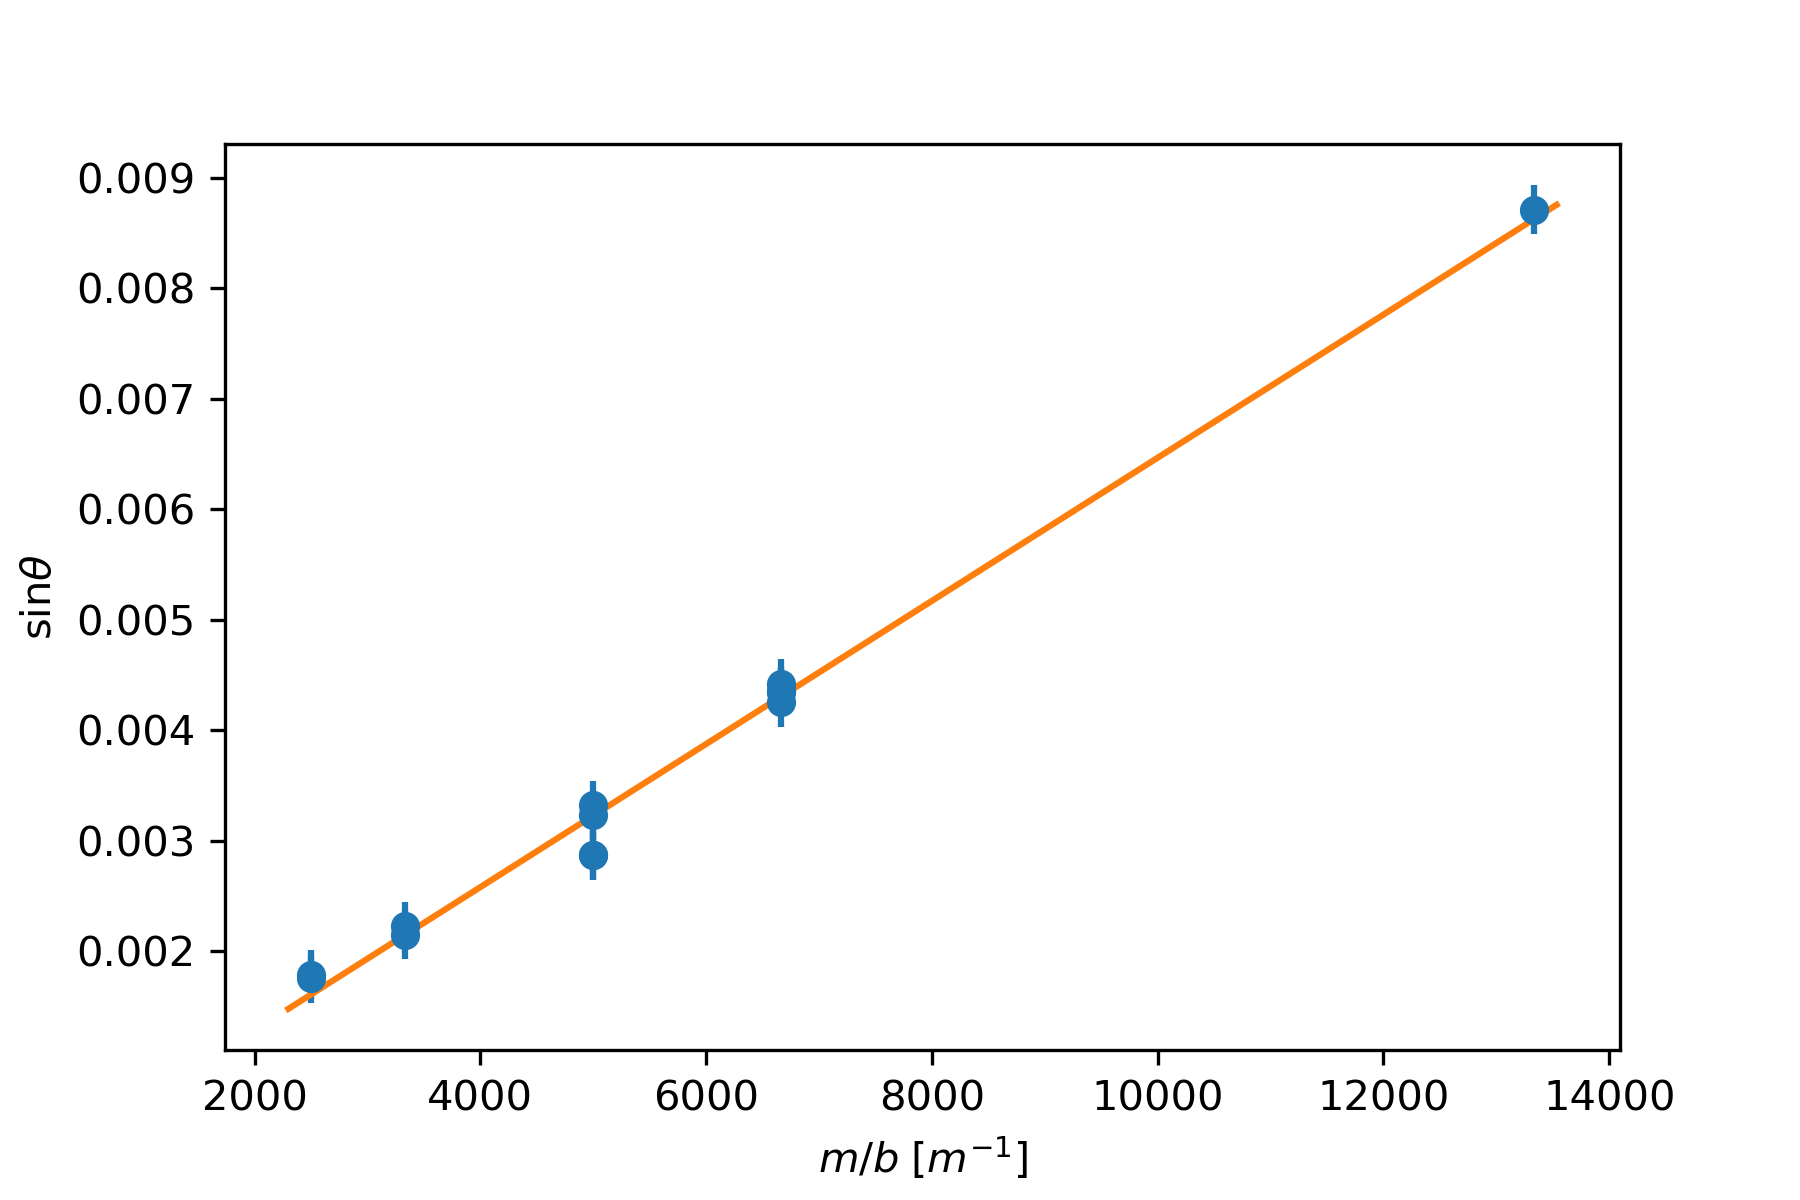
\includegraphics[width=1.1\linewidth]{fitFenditura.png}
	\captionof{figure}{Fit relativo alla sola fenditura}
	\label{fig:fitFenditura}
	\end{center}
\end{Figure}

Si ricava un valore del coefficiente angolare, ossia della lunghezza d'onda stimata, di
\[
\lambda^{\text{meas}} = \SI{648 \pm 18}{nm} = \SI{6.5 \pm 0.2 e-7}{m},
\]
compatibile con il valore dichiarato dal costruttore. 

Si ripete lo studio sui dati completi (fenditura ed apertura circolare). Il grafico, in Figura~\ref{fig:slit-circ}, è riportato in funzione della variabile indipendente $m\times c(m)/b$, in modo da includere i fattori moltiplicativi dati dai coefficienti di Bessel. 
\begin{Figure}
	\begin{center}
	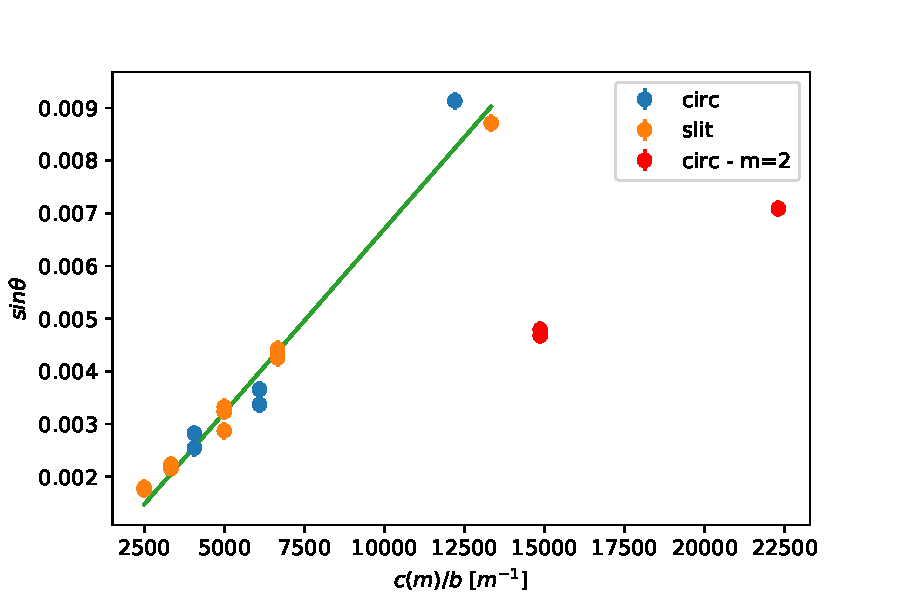
\includegraphics[width=1.1\linewidth]{slit-circ}
	\captionof{figure}{Fit sui dati relativi alla fenditura (\emph{slit}) e all'apertura circolare (\emph{circ}).}
	\label{fig:slit-circ}
	\end{center}
\end{Figure}
Il fit lineare sulle variabili $(x-x_0)/L$ e $m \times c(m)/b$ è stato eseguito scartando dai dati riferiti all'apertura circolare quelli riguardanti il minimo di ordine $m=2$ (riportati in rosso nel grafico) in quanto inattendibili rispetto all'andamento degli altri punti. Si ritiene che la stima di tali minimi sia stata viziata da una luminosità di fondo comparabile con il segnale d'interesse; inoltre, si ritiene che, poiché il fotodiodo compie una misura integrata sull'intera area della propria regione sensibile di diametro $\approx \SI{200}{\micro m}$ e non invece una misura puntuale, l'individuazione del minimo osservando solo l'andamento della tensione ai suoi capi possa essere stata inaccurata. 

Si ricava un valore del coefficiente angolare, ossia della lunghezza d'onda stimata, di
\[
\lambda^{\text{meas}} = \SI{697 \pm 28}{nm} = \SI{7.0 \pm 0.3 e-7}{m},
\]
compatibile, entro due deviazioni standard, con il valore dichiarato dal costruttore e con quello stimato in precedenza. Si propone dunque come miglior stima della lunghezza d'onda del laser la media pesata delle due misure
\[
\bar \lambda = \SI{678 \pm 33}{nm} = \SI{6.8 \pm 0.3 e-7}{m},
\]
compatibile anch'essa entro due deviazioni standard con il valore previsto dal costruttore.

\section{Ricostruzione dell'intera figura di diffrazione per una fenditura}\label{sec:figura_di_diffrazione}

Si ricostruisce l'intera figura di diffrazione per una fenditura di $\SI{300}{\micro m}$. L'analisi nell'approssimazione di Fraunhofer della diffrazione da parte di una fenditura di un'onda monocromatica fornisce la seguente formula per l'intensità:
\begin{equation}\label{eq:slit_diffraction_figure}
I(x) = I_0\left (\frac{\sin\left(\frac{\pi xa}{\lambda z}\right)}{\frac{\pi xa}{\lambda z}}\right)^2,
\end{equation}
dove $z = \SI{90.0 \pm 0.2}{cm}$ è la distanza del fotodiodo dalla fenditura, $a$ è l'apertura della fenditura e $x$ è la posizione di rivelazione perpendicolare alla direzione di propagazione della radiazione.
Si prendono punti a intervalli regolari di \SI{100}{\micro m} l'uno dall'altro. Le misure sono riportate in Tabella \ref{tab:interaFenditura} in Appendice, mentre in Figura \ref{fig:I} è riportato il grafico dei dati con sovrapposta la curva di fit usando come parametro libero l'apertura della fenditura. Il fit per la lunghezza d'onda fornisce il valore
\[
 \lambda = \SI{570 \pm 20}{nm} = \SI{5.7 \pm 0.2 e-7}{m},
\]
non compatibile con il valore dichiarato dal costruttore e con il valore stimato nella sezione precedente. Si identificano due possibili cause di errore:
\begin{itemize}[label={-}]
\item L'equazione per l'intensità è ricavata supponendo che la radiazione incidente sia un'onda piana monocromatica. In realtà il fascio diffratto è gaussiano e si ipotizza che la sua convoluzione in Fraunhofer con la fenditura porti a un'allargamento della figura di diffrazione, con conseguente sottostima di $\lambda$.
\item La dimensione della fenditura non coincide con quella dichiarata dal costruttore. Effettuiamo dunque un fit sui dati sperimentali e troviamo $$a = \SI{237 \pm 1}{\micro m},$$ corrispondente a un errore del 21\% sul valore dichiarato.
\end{itemize}

\begin{Figure}
	\begin{center}
	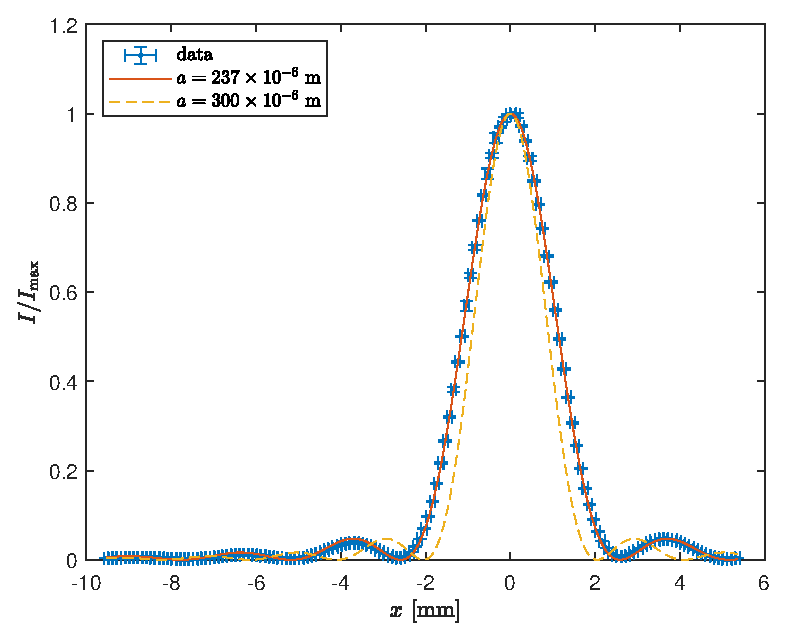
\includegraphics[width=\linewidth]{figura_diffrazione.eps}
	\captionof{figure}{Dati sperimentali con sovrapposta curva di fit avente lo spessore della fenditura come parametro e curva teorica attesa; $\lambda = \SI{632.8}{nm}$. }
	\label{fig:I}
	\end{center}
\end{Figure}


\section{Verifica del principio di Babinet e misura del diametro di un capello}
Si sostituisce la fenditura con un capello umano, per il \emph{Principio di Babinet} la figura di diffrazione teorica prodotta coincide con quella di una fenditura di apertura pari allo spessore $d$ del capello\footnote{Nel dire questo si è assunto che il capello abbia forma parallelepipeda, e non cilindrica, orientato in modo che due facce siano perpendicolari al vettore d'onda del fascio laser.}, come descritto in (\ref{eq:slit_diffraction_figure}). 

Misurando l'intensità del fascio al variare della distanza $x$ dal massimo si trovano le misure riportate in Figura~\ref{fig:babinet} e in Tabella~\ref{tab:babinet}, in Appendice. Nella stessa figura è riportato il fit dell'andamento teorico dove il parametro libero è lo spessore $d$ e la lunghezza d'onda è quella dichiarata dal costruttore, ovvero $\lambda = \SI{632.8}{nm}$.
\begin{Figure}
	\begin{center}
	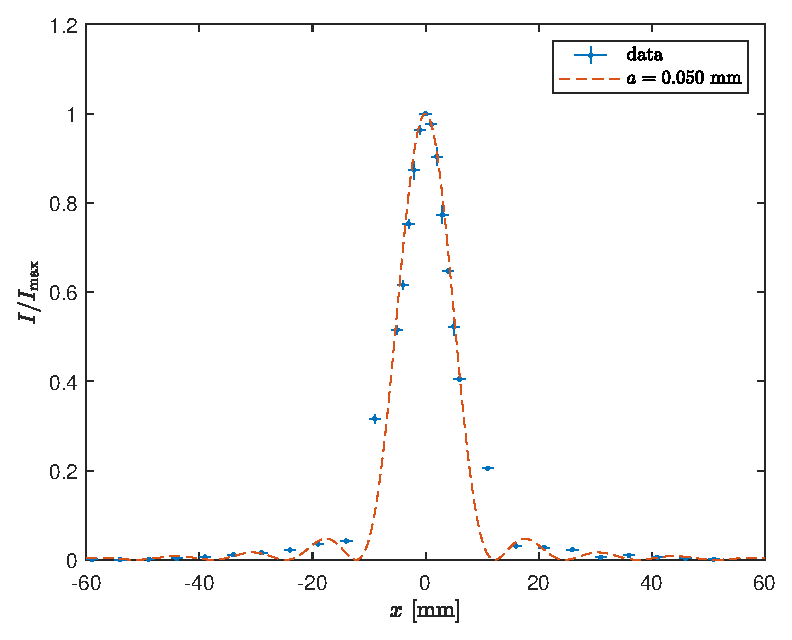
\includegraphics[width=\linewidth]{babinet.eps}
	\captionof{figure}{Dati sperimentali relativi al capello, con sovrapposta curva di fit.}
	\label{fig:babinet}
	\end{center}
\end{Figure}

Dal fit si ricava uno spessore del capello pari a 
\[
	d = \SI{0.050 \pm 0.003}{mm},
\]
compatibile con le dimensioni medie previste per un capello.

Il fit è stato ottenuto pesando i dati della campana centrale dieci volte in più rispetto ai punti sulle code: questa scelta è dovuta al fatto che l'andamento che si è ritenuto più significativo è quello centrale, poiché i punti sono stati presi con densità troppo bassa per interpolare correttamente i minimi; inoltre non si può essere completamente sicuri che il capello fosse perpendicolare alla direzione di spostamento del fotodiodo e che il laser fosse ben allineato, dunque la figura di interferenza risulta, com'era prevedibile, asimmetrica. 

\section{Conclusioni}
Il valore della lunghezza d'onda stimato utilizzando solamente i dati della fenditura risulta essere più accurato rispetto a quello ottenuto dalle misure di diffrazione per fenditura e apertura circolare. Si ritiene che questo sia dovuto al diverso grado di accuratezza della trattazione come onda piana del fascio laser. Essendo esso, infatti, un fascio gaussiano, origina figure di diffrazione diverse, che dipendono non solo dalla forma dell'apertura, ma anche dal posizionamento della stessa rispetto all'asse del fascio, nonché dall'allineamento con l'asse lungo cui viene spostato il fotodiodo.

Ulteriore sorgente di incertezza riguarda la misura fatta dal fotodiodo mediando sulla regione attiva, in contrasto con l'andamento puntuale ricavato teoricamente. Si ritiene che anche l'intensità del fondo, comparabile in diversi casi con il valore del minimo, possa averne influenzato l'identificazione e la misura.

Infine, si osserva che il \emph{Principio di Babinet} è soddisfatto utilizzando un capello umano, e tenendo conto di sistematiche sperimentali dovute al non corretto allineamento e alla forma tridimensionale dello stesso.





\end{multicols}


\newpage
\section{Appendice}


\begin{minipage}[t]{.5\linewidth}
\vspace{0cm}
\begin{center}
\captionof{table}{Misure di diffrazione attraverso la fenditura.}
\label{tab:misuraLambda1}
\begin{tabular}{c|c|c|c}
$m$ & $b$ [\SI{}{mm}] & $x_0$ [\SI{}{mm}] & $x-x_0$ [\SI{}{mm}]\\
 & & $\pm 0.1$ & $\pm 0.2$\\
\hline
  1 & 0.2 & 4.3 &  2.6 \\
 -1 & 0.2 & 4.3 & -2.6 \\
  1 & 0.3 & 8.6 & -2.0 \\
 -1 & 0.3 & 8.6 &  2.0 \\
  2 & 0.3 & 8.6 & -3.9 \\
 -2 & 0.3 & 8.6 &  3.8 \\
  1 & 0.4 & 8.5 &  1.6 \\
  2 & 0.4 & 8.5 &  3.0 \\
 -1 & 0.4 & 8.5 & -1.6 \\
 -2 & 0.4 & 8.5 & -2.9 \\
  1 & 0.1 & 8.6 &  3.9 \\
 -1 & 0.1 & 8.6 & -4.0 \\
 -2 & 0.1 & 8.6 & -7.8 \\
\hline
\end{tabular}
\end{center}
\end{minipage}
\quad
\begin{minipage}[t]{.5\linewidth}
\vspace{0cm}
\begin{center}
\captionof{table}{Misure di diffrazione attraverso l'apertura circolare.}
\label{tab:misuraLambda2}
\begin{tabular}{c|c|c|c}
$m \times c(m)$ & $b$ [\SI{}{mm}] & $x_0$ [\SI{}{mm}] & $x-x_0$ [\SI{}{mm}]\\
 & & $\pm 0.1$ & $\pm 0.2$\\
\hline
  $1 \times 1.22$ & 0.3 & 9.8 &  2.5 \\
  $2 \times 2.23$ & 0.3 & 9.8 &  4.3 \\
 $-1 \times 1.22$ & 0.3 & 9.8 & -2.3 \\
 $-2 \times 2.23$ & 0.3 & 9.8 & -4.2 \\
 $-1 \times 1.22$ & 0.1 & 9.6 & -8.2 \\
 $1 \times 1.22$ & 0.2 & 9.6 &  3.0 \\
 $-1 \times 1.22$ & 0.2 & 9.6 & -3.3 \\
 $-2 \times 2.23$ & 0.2 & 9.6 & -6.4 \\
\hline
\end{tabular}
\end{center}
\end{minipage}

\vspace{1cm}

\captionof{table}{Misure per l'intero pattern di diffrazione da una fenditura, $b=\SI{300}{\micro m}$.}
\label{tab:interaFenditura}
\begin{minipage}{0.33\linewidth}
\begin{center}
\begin{tabular}{c|c|c}
$x$ [\SI{}{mm}] & $V$ [\SI{}{V}] & $\sigma_V$ [\SI{}{V}] \\
 $\pm 0.1$ & & \\
\hline
 0.1 & 0.028 & 0.001 \\
  0.2 & 0.032 & 0.001 \\
  0.3 & 0.036 & 0.001 \\
  0.4 & 0.040 & 0.001 \\
  0.5 & 0.044 & 0.001 \\
  0.6 & 0.046 & 0.001 \\
  0.7 & 0.047 & 0.001 \\
  0.8 & 0.048 & 0.001 \\
  0.9 & 0.047 & 0.001 \\
  1.0 & 0.045 & 0.001 \\
  1.1 & 0.043 & 0.001 \\
  1.2 & 0.039 & 0.001 \\
  1.3 & 0.034 & 0.001 \\
  1.4 & 0.031 & 0.001 \\
  1.5 & 0.026 & 0.001 \\
  1.6 & 0.022 & 0.001 \\
  1.7 & 0.018 & 0.001 \\
  1.8 & 0.015 & 0.001 \\
  1.9 & 0.013 & 0.001 \\
  2.0 & 0.013 & 0.001 \\
  2.1 & 0.015 & 0.001 \\
  2.2 & 0.019 & 0.001 \\
  2.3 & 0.024 & 0.001 \\
\hline
\end{tabular}
\end{center}
\end{minipage}
\begin{minipage}{0.33\linewidth}
\begin{center}
\begin{tabular}{c|c|c}
$x$ [\SI{}{mm}] & $V$ [\SI{}{V}] & $\sigma_V$ [\SI{}{V}] \\
 $\pm 0.1$ & & \\
\hline
  2.4 & 0.031 & 0.001 \\
  2.5 & 0.039 & 0.001 \\
  2.6 & 0.049 & 0.001 \\
  2.7 & 0.058 & 0.001 \\
  2.8 & 0.068 & 0.001 \\
  2.9 & 0.078 & 0.001 \\
  3.0 & 0.087 & 0.001 \\
  3.1 & 0.094 & 0.001 \\
  3.2 & 0.098 & 0.001 \\
  3.3 & 0.101 & 0.001 \\
  3.4 & 0.101 & 0.001 \\
  3.5 & 0.100 & 0.001 \\
  3.6 & 0.094 & 0.001 \\
  3.7 & 0.086 & 0.001 \\
  3.8 & 0.077 & 0.001 \\
  3.9 & 0.066 & 0.001 \\
  4.0 & 0.055 & 0.001 \\
  4.1 & 0.044 & 0.001 \\
  4.2 & 0.034 & 0.001 \\
  4.3 & 0.027 & 0.001 \\
  4.4 & 0.022 & 0.001 \\
  4.5 & 0.022 & 0.001 \\
  4.6 & 0.026 & 0.001 \\
\hline
\end{tabular}
\end{center}
\end{minipage}
\begin{minipage}{0.33\linewidth}
\begin{center}
\begin{tabular}{c|c|c}
$x$ [\SI{}{mm}] & $V$ [\SI{}{V}] & $\sigma_V$ [\SI{}{V}] \\
 $\pm 0.1$ & & \\
\hline
  4.7 & 0.035 & 0.001 \\
  4.8 & 0.050 & 0.001 \\
  4.9 & 0.070 & 0.001 \\
  5.0 & 0.092 & 0.001 \\
  5.1 & 0.121 & 0.001 \\
  5.2 & 0.153 & 0.001 \\
  5.3 & 0.188 & 0.001 \\
  5.4 & 0.221 & 0.001 \\
  5.5 & 0.256 & 0.001 \\
  5.6 & 0.285 & 0.001 \\
  5.7 & 0.308 & 0.002 \\
  5.8 & 0.323 & 0.001 \\
  5.9 & 0.334 & 0.001 \\
  6.0 & 0.334 & 0.001 \\
  6.1 & 0.323 & 0.001 \\
  6.2 & 0.304 & 0.001 \\
  6.3 & 0.277 & 0.001 \\
  6.4 & 0.239 & 0.001 \\
  6.5 & 0.197 & 0.001 \\
  6.6 & 0.153 & 0.001 \\
  6.7 & 0.110 & 0.001 \\
  6.8 & 0.072 & 0.001 \\
  6.9 & 0.047 & 0.001 \\
\hline
\end{tabular}
\end{center}
\end{minipage}

\begin{minipage}[t]{0.33\linewidth}
\vspace{0cm}
\begin{center}
\begin{tabular}{c|c|c}
$x$ [\SI{}{mm}] & $V$ [\SI{}{V}] & $\sigma_V$ [\SI{}{V}] \\
 $\pm 0.1$ & & \\
\hline
  7.0 & 0.034 & 0.001 \\
  7.1 & 0.043 & 0.001 \\
  7.2 & 0.080 & 0.001 \\
  7.3 & 0.156 & 0.001 \\
  7.4 & 0.262 & 0.002 \\
  7.5 & 0.41 & 0.01 \\
  7.6 & 0.61 & 0.01 \\
  7.7 & 0.85 & 0.01 \\
  7.8 & 1.15 & 0.01 \\
  7.9 & 1.50 & 0.01 \\
  8.0 & 1.90 & 0.02 \\
  8.1 & 2.34 & 0.02 \\
  8.2 & 2.81 & 0.01 \\
  8.3 & 3.35 & 0.05 \\
  8.4 & 3.90 & 0.02 \\
  8.5 & 4.40 & 0.01 \\
 8.6 & 5.00 & 0.10 \\
  8.7 & 5.60 & 0.05 \\
  8.8 & 6.15 & 0.05 \\
  8.9 & 6.67 & 0.01 \\
  9.0 & 7.17 & 0.02 \\
  9.1 & 7.60 & 0.10 \\
  9.2 & 7.96 & 0.05 \\
  9.3 & 8.30 & 0.09 \\
  9.4 & 8.52 & 0.02 \\
  9.5 & 8.66 & 0.05 \\
  9.6 & 8.75 & 0.02 \\
  9.7 & 8.78 & 0.02 \\
  9.8 & 8.75 & 0.05 \\
  9.9 & 8.53 & 0.02 \\
 10.0 & 8.25 & 0.02 \\
 10.1 & 7.90 & 0.05 \\
 10.2 & 7.46 & 0.02 \\
 10.3 & 7.00 & 0.01 \\
 10.4 & 6.52 & 0.01 \\
 10.5 & 5.97 & 0.02 \\
 10.6 & 5.46 & 0.02 \\
 10.7 & 4.92 & 0.02 \\
 10.8 & 4.34 & 0.02 \\
 10.9 & 3.75 & 0.02 \\
 11.0 & 3.20 & 0.01 \\
\hline
\end{tabular}
\end{center}
\end{minipage}
\begin{minipage}[t]{0.33\linewidth}
\vspace{0cm}
\begin{center}
\begin{tabular}{c|c|c}
$x$ [\SI{}{mm}] & $V$ [\SI{}{V}] & $\sigma_V$ [\SI{}{V}] \\
 $\pm 0.1$ & & \\
\hline
 11.1 & 2.70 & 0.02 \\
 11.2 & 2.24 & 0.01 \\
 11.3 & 1.80 & 0.01 \\
 11.4 & 1.41 & 0.01 \\
 11.5 & 1.09 & 0.01 \\
 11.6 & 0.80 & 0.01 \\
 11.7 & 0.56 & 0.01 \\
 11.8 & 0.370 & 0.002 \\
 11.9 & 0.232 & 0.002 \\
 12.0 & 0.140 & 0.002 \\
 12.1 & 0.085 & 0.001 \\
 12.2 & 0.060 & 0.001 \\
 12.3 & 0.064 & 0.001 \\
 12.4 & 0.088 & 0.001 \\
 12.5 & 0.130 & 0.001 \\
 12.6 & 0.175 & 0.001 \\
 12.7 & 0.231 & 0.001 \\
 12.8 & 0.285 & 0.002 \\
 12.9 & 0.328 & 0.001 \\
 13.0 & 0.365 & 0.001 \\
 13.1 & 0.394 & 0.002 \\
 13.2 & 0.406 & 0.002 \\
 13.3 & 0.412 & 0.002 \\
 13.4 & 0.404 & 0.002 \\
 13.5 & 0.385 & 0.001 \\
 13.6 & 0.360 & 0.001 \\
 13.7 & 0.325 & 0.001 \\
 13.8 & 0.286 & 0.001 \\
 13.9 & 0.244 & 0.001 \\
 14.0 & 0.201 & 0.001 \\
 14.1 & 0.157 & 0.001 \\
 14.2 & 0.119 & 0.001 \\
 14.3 & 0.086 & 0.001 \\
 14.4 & 0.060 & 0.001 \\
 14.5 & 0.036 & 0.001 \\
 14.6 & 0.022 & 0.001 \\
 14.7 & 0.016 & 0.001 \\
 14.8 & 0.016 & 0.001 \\
 14.9 & 0.021 & 0.001 \\
 15.0 & 0.031 & 0.001 \\
\hline
\end{tabular}
\end{center}
\end{minipage}
\begin{minipage}[t]{0.33\linewidth}
\vspace{0cm}
\begin{center}
\captionof{table}{Misure di diffrazione per un capello.}
\label{tab:babinet}
\begin{tabular}{c|c|c}
$x$ [\SI{}{mm}] & $V$ [\SI{}{V}] & $\sigma_V$ [\SI{}{V}]\\
$\pm 0.1$ & & \\
\hline
 15.0 & 0.011 & 0.001 \\
 14.5 & 0.031 & 0.001 \\
 14.0 & 0.057 & 0.001 \\
 13.5 & 0.098 & 0.001 \\
 13.0 & 0.058 & 0.001 \\
 12.5 & 0.228 & 0.001 \\
 12.0 & 0.274 & 0.001 \\
 11.5 & 0.308 & 0.002 \\
 11.0 & 2.040 & 0.010 \\
 10.5 & 4.03 & 0.03 \\
  10.4 & 5.2 & 0.1 \\
 10.3 & 6.45 & 0.03 \\
 10.2 & 7.7 & 0.1 \\
  10.1 & 9.0 & 0.1 \\
 10.0 & 9.7 & 0.1 \\
   9.9 & 9.96 & 0.01 \\
  9.8 & 9.60 & 0.05 \\
  9.7 & 8.7 & 0.1 \\
  9.6 & 7.50 & 0.05 \\
  9.4 & 5.130 & 0.001 \\
  9.5 & 6.130& 0.05 \\
  9.0 & 3.150& 0.05 \\
  8.5 & 0.420& 0.01 \\
  8.0 & 0.352 & 0.002 \\
  7.5 & 0.219 & 0.001 \\
  7.0 & 0.155 & 0.001 \\
  6.5 & 0.110 & 0.001 \\
  6.0 & 0.062 & 0.001 \\
  5.5 & 0.030 & 0.001 \\
  5.0 & 0.011 & 0.001 \\
  4.5 & 0.006 & 0.001 \\
  4.0 & 0.008 & 0.001 \\
\hline
\end{tabular}
\end{center}
\end{minipage}









%ESEMPIO DI FIGURA
%\begin{Figure}
%	\begin{center}
%	\includegraphics[width=\linewidth]{comune.png}
%	\captionof{figure}{Istantanea dell'oscilloscopio per l'amplificatore differenziale, misura di $A_c$}
%	\label{fig:Ac_differenziale}
%	\end{center}
%\end{Figure}


%ESEMPIO DI TABELLA
%\begin{center}
%\captionof{table}{Misure per la stima di $A_c$}
%\label{tab:Ac_differenziale}
%\begin{tabular}{c|c|c|c}
%$f$ [\SI{}{Hz}] & $V_i$ [\SI{}{V}] & $v_o$ [\SI{}{mV}] & $A_c = v_o / V_i$ \\
%\hline
%      149.5 &        3.90 &         11.3 & 2.90e-03 \\
%      222.0 &        3.90 &         11.5 & 2.95e-03 \\
%      281.0 &        3.90 &         11.8 & 3.03e-03 \\
%      359.0 &        3.90 &         11.8 & 3.03e-03 \\
%      461.0 &        3.90 &         12.2 & 3.13e-03 \\
%\hline
%\end{tabular}
%\end{center}


\end{document}
